% vim: set tabstop=4 :

\newcommand{\figtb}[5]{ %引数 {日本語タイトル}{英語タイトル}{サイズ}{ファイル名}{ラベル名}
\begin{figure}[tb]
  \begin{center}
    \includegraphics[width=#3cm,clip]{figure/#4}
    \caption{#1}
    \ecaption{#2}
    \label{fig:#5}
  \end{center}
\end{figure}}
\newcommand{\eq}[1]{式(\ref{eq:#1})}
%**********************************************************
\chapter{人流シミュレーション}
%\chapter{本来なら問題定義や背景的な何かを書く}
\label{sec:background}
%**********************************************************
人流シミュレーションは,コンピュータ上で人の動きを再現する手法であり,
図\ref{fig:jinryu_image}に人流シミュレーションの例を示す.
図\ref{fig:jinryu_image}中の
青色の丸は右側に進む人,緑色の丸は左側に進む人,黄色の四角は壁,青色の四角
は障害物である.
赤色の障害物は,自動販売機やゴミ箱などの移動が可能である設置物である.
図\ref{fig:jinryu_image}の例では,通路が赤色の障害物によって通路が狭くなっている
ため,人の滞留や混雑が起きているため,赤色の障害物を撤去することで滞留や
混雑を防ぐことができる.
図\ref{fig:jinryu_image}のような混雑や滞留を発見するためには,実際に多くの人で
実験する必要があるため,時間や費用がかかる.一方で,
人流シミュレーションは,コンピュータ上で再現できることから
,実際に多くの人を用いて実験するよりも,必要な時間や金額を抑えることが可能である.
このように,人流シミュレーションの目的は,人の滞留や混雑が起きないように
対策することである.
このため,人流シミュレーションは,大規模なイベントを企画する企業や
大規模や施設を設計,建築する建設業などで活用されている(参考文献).
人流シミュレーションを活用することで,事前に人の流れを予測することが可能に
なり,地震や火災などの有事のときに,非常灯や看板の配置,警備員の配置などを
最適化できるため,適切な誘導が行うことが可能になる.
%人流シミュレーションに必要な要素
人流シミュレーションを用いて解析するためには,空間を再現するための
空間のモデル化,歩行者を再現するための歩行者のモデル化,障害物や壁を再現
するための障害物のモデル化が必要である.

\begin{figure}[h]
    \begin{center}
     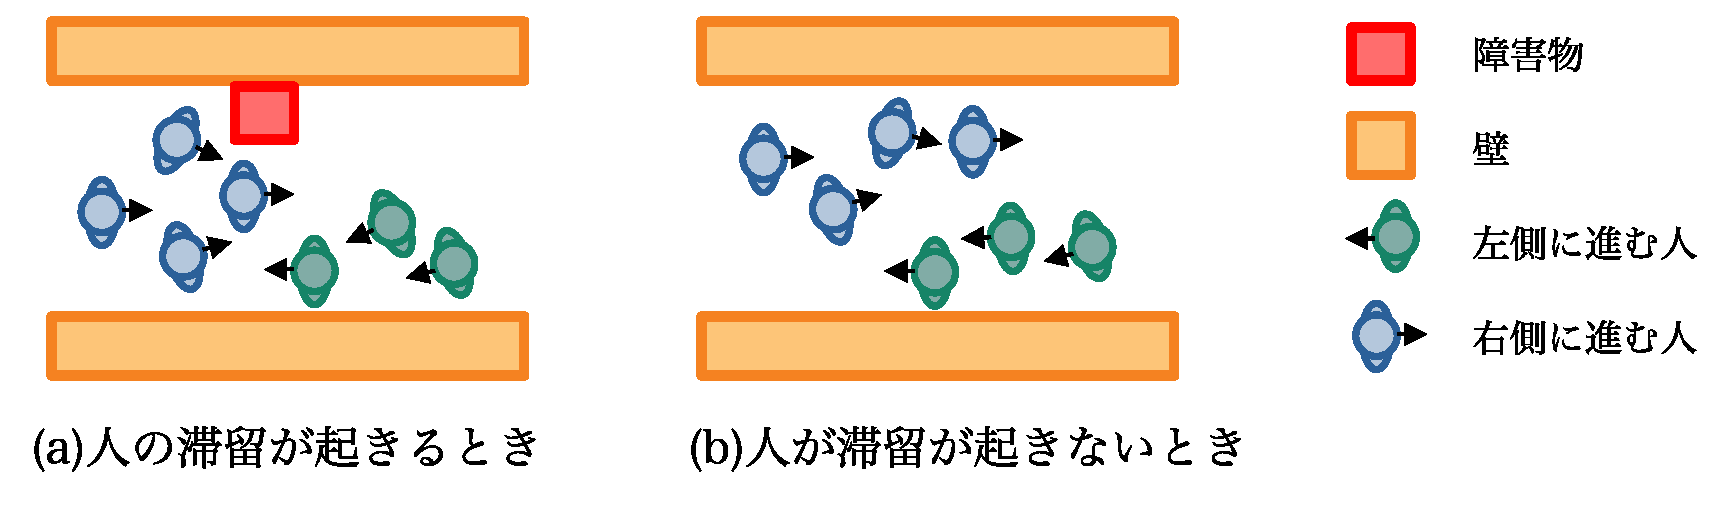
\includegraphics[width=14cm,clip]{figure/jinryu_image2_r2.eps}
     \caption{人流シミュレーションの活用例}
     \label{fig:jinryu_image}
    \end{center}
\end{figure}


\section{空間モデル}
空間モデルは,解析したい場所をコンピュータで計算するために,空間を離散化するための
ものである.
シミュレーション対象が海岸から近い都市や人口が多い都市などの道路上の人々の流れを解析するためには,
数千人から数万人の解析が可能なネットワークモデルが用いられる(参考文献).
また,シミュレーション対象が商業施設や駅構内などの施設上の人々を解析するためには,
フロアフィールドモデルや連続座標モデルが用いられる(参考文献).



\subsection{ネットワークモデル}
ネットワークモデルは,

\begin{figure}[h]
    \begin{center}
     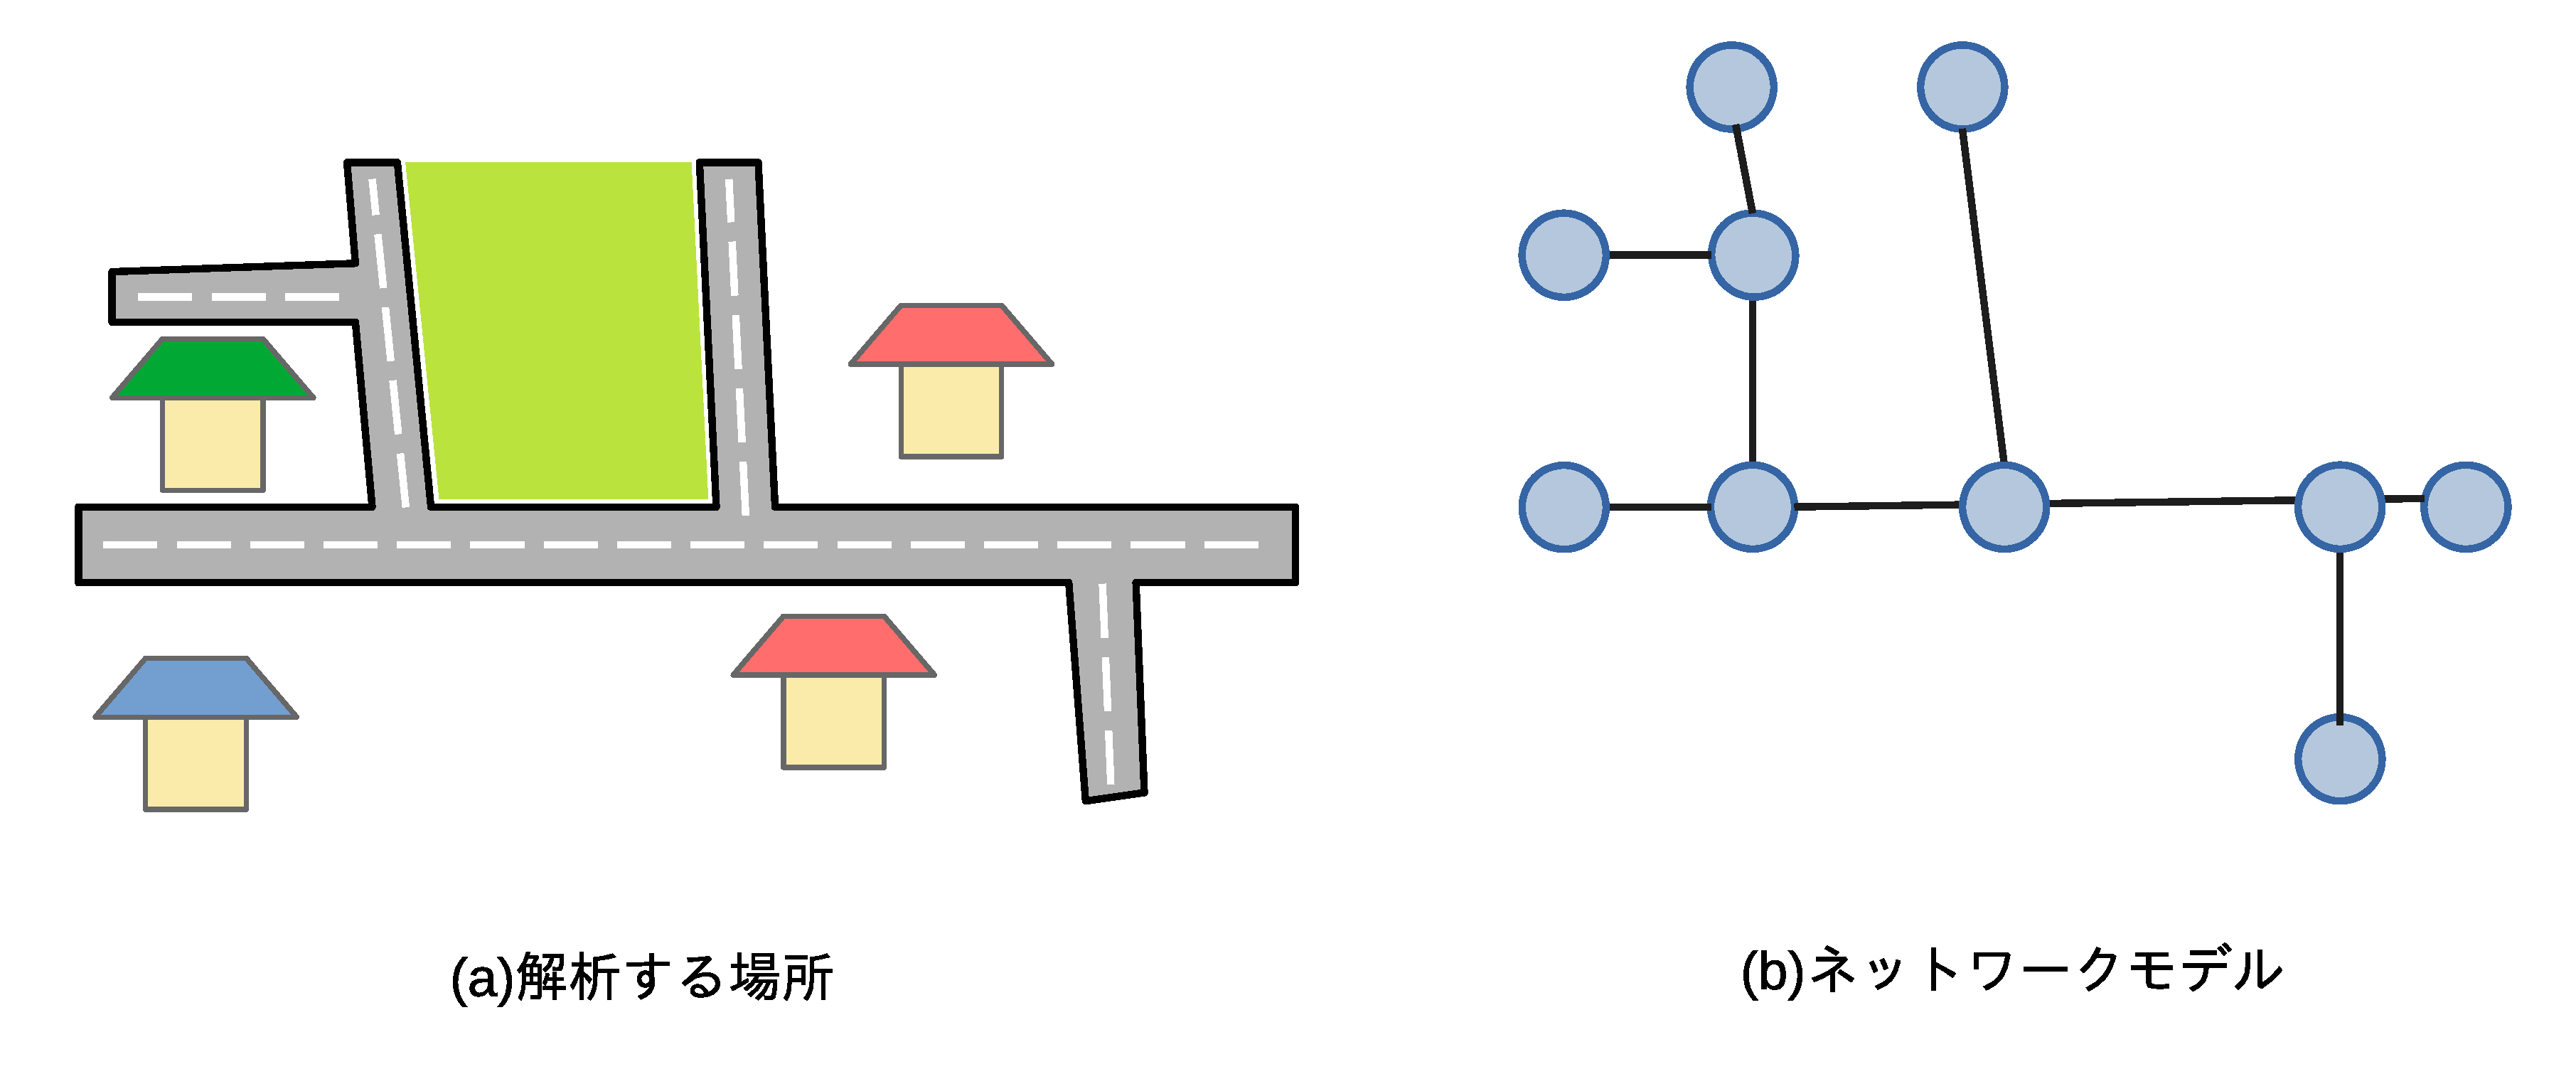
\includegraphics[width=14cm,clip]{figure/networkmodel_ex.eps}
     \caption{ネットワークモデルの例}
     \label{fig:jinryu_image2}
    \end{center}
\end{figure}


\subsection{フロアフィールドモデル}
フロアフィールドモデルは,


\subsection{連続座標モデル}
連続座標モデルは,


\begin{figure}[htbp]
    \begin{minipage}[b]{0.5\linewidth}
      \centering
      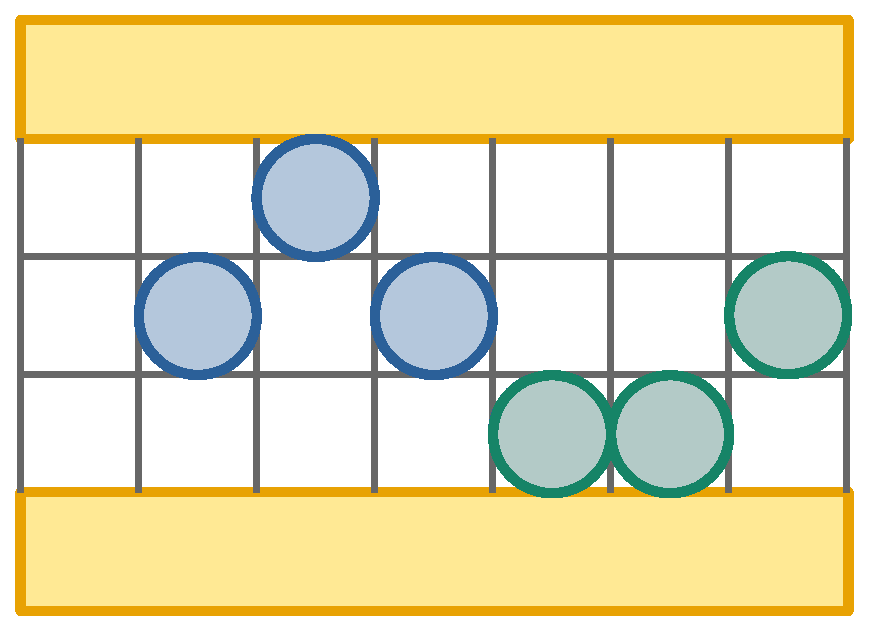
\includegraphics[keepaspectratio, scale=0.23]{figure/floormodel_ex.eps}
      \caption{フロアフィールドモデルの例}
      \label{fig:serumaton}
    \end{minipage}
    \begin{minipage}[b]{0.5\linewidth}
      \centering
      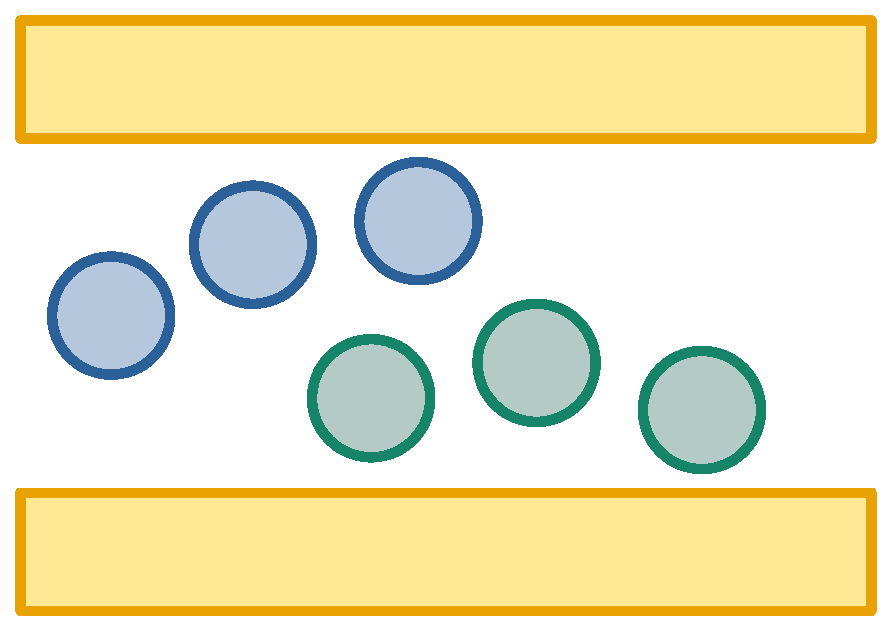
\includegraphics[keepaspectratio, scale=0.23]{figure/renzoku_model_ex.eps}
      \caption{二次元連続座標モデルの例}
      \label{fig:renzoku}
    \end{minipage}
\end{figure}

\section{歩行者モデル}
歩行者モデルは,人流シミュレーションの中で歩行者の動きを決定するモデルであり,


\subsection{ネットワークモデルの歩行者モデル**}

\subsection{静的フロアモデル}
静的フロアモデルは,図\ref{fig:serumaton}に示すようなフロアフィールドモデルの空間モデルを用いて
おり,格子ごとに目的地までの距離を設定し,確率を用いてエージェントを移動させることで解析する手法である.
図\ref{fig:huroa_model_image}に静的フロアフィールドモデルのイメージを示す.
図\ref{fig:huroa_model_image}中の格子は解析領域,青丸はエージェント,青色の矢印はエージェントの移動可能な
方向である.
図\ref{fig:huroa_model_image}のように,静的フロアフィールドモデルは,

\begin{figure}[h]
    \begin{center}
     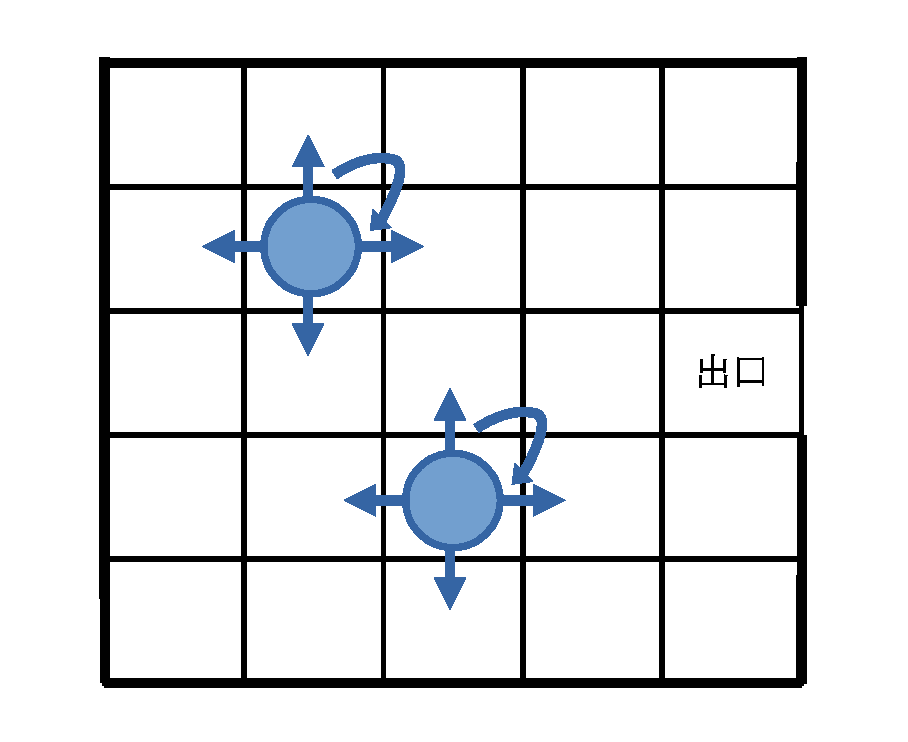
\includegraphics[width=14cm,clip]{figure/floormodel_image.eps}
     \caption{静的フロアフィールドモデルのイメージ}
     \label{fig:huroa_model_image}
    \end{center}
\end{figure}


図\ref{fig:huroa_model}に室内からの退出時における静的フロアフィールドの例を示す.
図\ref{fig:huroa_model}中の~~である.
図\ref{fig:huroa_model}中の(a)マンハッタン距離と(b)ユークリッド距離は,各格子から出口までの
距離を示す.
静的フロアフィールドモデルは,計算対象のエージェントの周囲のセルのなかから,出口までの
距離が小さくなるようなセルを選択することで,出口までの解析が可能となる.
静的フロアフィールドモデルの利点は,解析前に各格子の計算を事前にできるため,非常に高速な
解析が可能である点である.
一方で,静的フロアフィールドは,出口前に形成されるアーチ現象の再現度が低いことが知られている.
図\ref{fig:huroa_model_ketten}に静的フロアフィールドモデルを用いた場合の出口前に形成される
アーチ現象の例を示す.
図\ref{fig:huroa_model_ketten}中の~~~である.
静的フロアフィールドモデルは,図\ref{fig;ruroa_model_ketten}のように,格子に一人のみ入ることができる
ことから,動きが格子サイズに制約されるため,出口付近の再現度が低い.
フロアフィールドモデルを用いた解析では,〇〇や△△,□□を用いることで,解析精度の向上が行われている
が,格子サイズの成約から,精度の向上に上限がある.
このため,高い解析精度が必要な場合は,SocialForceMoel(SFM)のような
解析領域を連続座標で解析する手法が用いられることが多い




\subsection{SocialForceModel(SFM)}
SocialFroceModel(SFM)は,周囲の状況に基づいて生成した運動方程式を用いて時間ステップ$t$ごとに
エージェントの移動を決定する.
\eq{sfm_siki1}にエージェント$i$の運動方程式を示す.
%
\begin{eqnarray}
  m_i \frac{dv_i}{dt} = m_i \frac{v_i^0 e_i - v_i}{\tau_i}
  +\sum_{j(\neq i)}f_{ij}+\sum_{W}f_{iW}
  \label{eq:sfm_siki1}
\end{eqnarray}
%
\eq{sfm_siki1}中の
右辺第一項はエージェントが目的地へ進む力を表しており,
エージェント$i$の体重$m_i$,
希望速度$v_i^0$,
目的地までの単位ベクトル$e_i$,現在の速度ベクトル$v_i$,
時定数$\tau_i$に基づいて算出される.
右辺第二項は周囲のエージェントを避ける力であり,
$f_{ij}$はエージェント$i$とエージェント$j$の相互作用力である.
また,第三項は壁などの障害物を避ける力であり,
$f_{iW}$はエージェント$i$が壁などの障害物$W$から受ける力である.
$f_{ij}$や$f_{iW}$は,\eq{sfm_siki2}と\eq{sfm_siki3}から算出する.
%
\begin{eqnarray}
  f_{ij} =  \{A_i exp [\frac{r_{ij} - d_{ij}}{B_i}  ]
  + kg(r_{ij} - d_{ij})\} n_{ij} \\ \nonumber
  + \kappa g (r_{ij} - d_{ij}) \Delta
  v^t_{ij} t_{ij}
  \label{eq:sfm_siki2}
\end{eqnarray}
%
\begin{eqnarray}
  f_{iW} = \{A_i exp[\frac{r_{i} - d_{iW}}{B_i}]
  + kg(r_{i} - d_{iW})\} n_{iW} \\ \nonumber
  + \kappa g (r_{i} - d_{iW}) (v_i t_{iW}) t_{iW}
  \label{eq:sfm_siki3}
\end{eqnarray}
%
式中の$r_i$はエージェント$i$の体の半径,
$t_{iW}$はエージェント$i$と壁$W$の垂直ベクトル,
$n_{iW}$はエージェント$i$と壁$W$の衝突面の法線ベクトル,
$A_i$はエージェント$i$のインタラクション作用,
$B_i$はエージェント$i$の反発作用,
$k$は衝突時の反発力係数,
$\kappa$は衝突時の摩擦力係数
である.
$d_{ij}, t_{ij}, n_{ij}, r_{ij}, \Delta v_{ij}$は,
エージェント$i$,$j$間の距離,
衝突面の垂直ベクトル,衝突面の法線ベクトル,体の半径の和,接線速度の差である.
また,衝突時関数$g(x)$は,\eq{gx_siki}に示すように$x$に応じてエージェント同士
の衝突を判定する.
%
\begin{equation}
  \label{eq:gx_siki}
  g(x) =
  \begin{cases}
    1 & (x<0)     \\
    0 & otherwise
  \end{cases}
\end{equation}
%
衝突時関数$g(x)$中の$x$は,エージェント同士の距離やエージェントと壁の距離であり,
衝突時であれば1,衝突していなければ0となる.




\section{障害物モデル}

\subsection{粒子によるモデル化}

\subsection{矩形によるモデル化}

\section{経路の設定}

\subsection{ダイクストラ法}



%1ブロックが10×30文字です
ああああああああああああああああああああああああああああああ
ああああああああああああああああああああああああああああああ
ああああああああああああああああああああああああああああああ
ああああああああああああああああああああああああああああああ
ああああああああああああああああああああああああああああああ
ああああああああああああああああああああああああああああああ
ああああああああああああああああああああああああああああああ
ああああああああああああああああああああああああああああああ
ああああああああああああああああああああああああああああああ
ああああああああああああああああああああああああああああああ
%
ああああああああああああああああああああああああああああああ
ああああああああああああああああああああああああああああああ
ああああああああああああああああああああああああああああああ
ああああああああああああああああああああああああああああああ
ああああああああああああああああああああああああああああああ
ああああああああああああああああああああああああああああああ
ああああああああああああああああああああああああああああああ
ああああああああああああああああああああああああああああああ
ああああああああああああああああああああああああああああああ
ああああああああああああああああああああああああああああああ
%
Penguin
ああああああああああああああああああああああああああああああ
ああああああああああああああああああああああああああああああ
ああああああああああああああああああああああああああああああ
ああああああああああああああああああああああああああああああ
ああああああああああああああああああああああああああああああ
ああああああああああああああああああああああああああああああ
ああああああああああああああああああああああああああああああ
ああああああああああああああああああああああああああああああ
ああああああああああああああああああああああああああああああ
ああああああああああああああああああああああああああああああ
%
ああああああああああああああああああああああああああああああ
ああああああああああああああああああああああああああああああ
ああああああああああああああああああああああああああああああ
ああああああああああああああああああああああああああああああ
ああああああああああああああああああああああああああああああ
ああああああああああああああああああああああああああああああ
ああああああああああああああああああああああああああああああ
ああああああああああああああああああああああああああああああ
ああああああああああああああああああああああああああああああ
ああああああああああああああああああああああああああああああ
%
ああああああああああああああああああああああああああああああ
ああああああああああああああああああああああああああああああ
ああああああああああああああああああああああああああああああ
ああああああああああああああああああああああああああああああ
ああああああああああああああああああああああああああああああ
ああああああああああああああああああああああああああああああ
ああああああああああああああああああああああああああああああ
ああああああああああああああああああああああああああああああ
ああああああああああああああああああああああああああああああ
ああああああああああああああああああああああああああああああ
ああああああああああああああああああああああああああああああ
%
ああああああああああああああああああああああああああああああ
ああああああああああああああああああああああああああああああ
ああああああああああああああああああああああああああああああ
ああああああああああああああああああああああああああああああ
ああああああああああああああああああああああああああああああ
ああああああああああああああああああああああああああああああ
ああああああああああああああああああああああああああああああ
ああああああああああああああああああああああああああああああ
ああああああああああああああああああああああああああああああ
%
ああああああああああああああああああああああああああああああ
ああああああああああああああああああああああああああああああ
ああああああああああああああああああああああああああああああ
ああああああああああああああああああああああああああああああ
ああああああああああああああああああああああああああああああ
ああああああああああああああああああああああああああああああ
ああああああああああああああああああああああああああああああ
ああああああああああああああああああああああああああああああ
ああああああああああああああああああああああああああああああ
ああああああああああああああああああああああああああああああ
%
ああああああああああああああああああああああああああああああ
ああああああああああああああああああああああああああああああ
ああああああああああああああああああああああああああああああ
ああああああああああああああああああああああああああああああ
ああああああああああああああああああああああああああああああ
あああああああああああああああああああああ
あああああああああああああああああああああ
%
%\chapter{背景(1671文字)}

%***** END ************************************************
